\documentclass[tikz]{standalone}


\usepackage{tikz}
\usetikzlibrary{calc}

\begin{document}
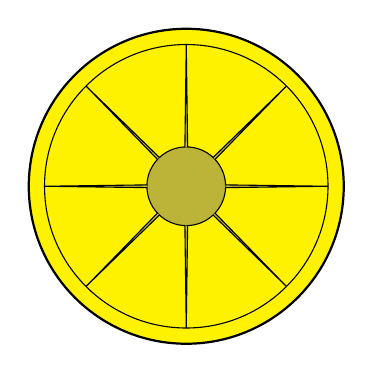
\begin{tikzpicture}[scale=2]

%\foreach \x in {-5,-4, ...,5}{
%	\draw[help lines] (\x,-5)node[below]{\x} -- (\x,5);
%}
%\foreach \y in {-5,-4, ...,5}{
%	\draw[help lines] (-5,\y)node[left]{\y} -- (5,\y);
%}


\def\r{.25}
\draw[fill=yellow, thick] (0,0)circle(1);
\draw[] (0,0)circle(.9);
\draw[fill=yellow!70!black] (0,0)circle(\r);


\foreach \alp in {0, 45, ..., 315}{
	\draw[fill=yellow!70!black] 
	(0,0)++(\alp+2:\r)--(\alp:.9)--(\alp-2:\r);
}





\end{tikzpicture}
\end{document}